\section{Definitions}

Formalization of a Tetris game and definition of the problem. A \emph{Tetris game} will refer to the hole game with its rules, conditions,... and a \emph{tetris match} will refer to a concrete Tetris game instance (no se com dir-ho). We will follow the formalization from \cite{TIH}.


\begin{definition}
  A \emph{board} B is an $n$ by $m$ grid. Each cell $\cell$, $i = 1\dots n$, $j = 1\dots m$ is \emph{filled} or \emph{unfilled}.
\end{definition}

The board will be indexed from bottom to top and from left to right. The cell $\cell[1][1]$ is in the bottom left of the board and $\cell[n][m]$ is the top right-most cell.\\

The following definitions will define the pieces and how they interact with the board.

\begin{definition}
  A \emph{piece type} $t$ is one of the following:$\ALL$. 
\end{definition}

\begin{definition}
 A \emph{piece state} in a board $B$ is a tuple $ P = \piece$ where:
  \begin{itemize}
    \item $t$ is a piece type
    \item $\theta$ is the \emph{orientation}, the number of degrees clockwise from the original piece. $ \theta \in \lbrace 0^\circ, 90^\circ, 180^\circ, 270^\circ \rbrace$. The Figure~\ref{allpieces} shows all the pieces and its rotations.
    \item $\cell$ is the \emph{position} of the piece in of $B$
    \item  $f$ indicates if the piece is \emph{fixed} or \emph{unfixed} in B.
  \end{itemize}

  We will refer to a piece sate as \emph{piece}.
   
\end{definition}


\begin{figure}[ht]
    \centering
    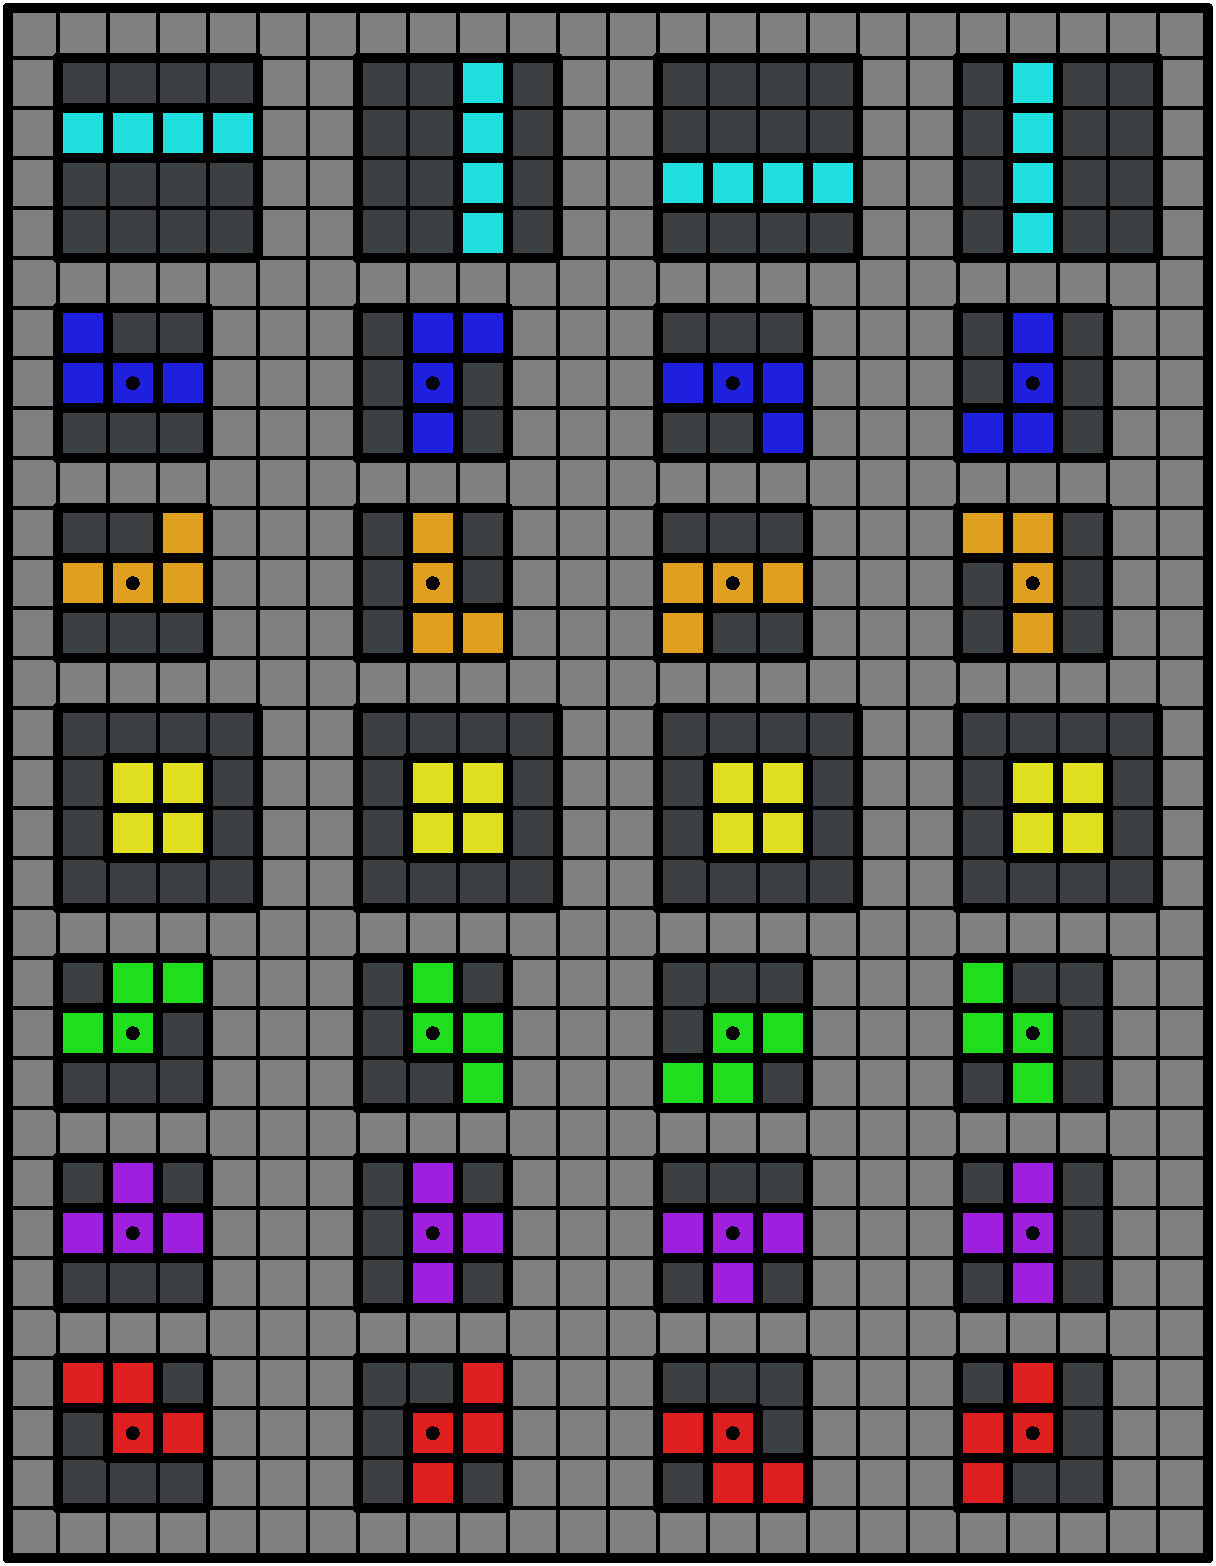
\includegraphics[width=160pt]{pieces/allpieces.pdf}
    \caption{All pieces, in order from top to bottom: $\II$, $\JJ$, $\LL$, $\OO$, $\SS$, $\TT$, $\ZZ$. The first column is the default orientation of a piece upon spawning in; each column to the right indicates a $90^\circ$ rotation clockwise about the rotation center of the piece.}
    \label{allpieces}
\end{figure}

\begin{definition}
  Given a piece type $t$ and a board $B$, the piece $P_0 = \piece[t][0^\circ][n][\lfloor m / 2 \rfloor][\text{unfixed}]$ is the \emph{initial state} of the piece type of $t$ in the board $B$.
\end{definition}

The idea is to have only one active piece in a Tetris match. Only the piece that is moving has a state because when a piece reaches the \emph{fixed} state the piece is automatically merged with the board, and then the next piece starts in its initial state. In order to define how a piece moves thought the board, we need to define some \emph{moves} for changing the piece state.

\begin{definition}
  A \emph{move} is a computable function $m(B, P) = P'$ that given a board $B$ and a piece $P$ outputs a new piece $P'$. The following moves can be applied to an unfixed piece $P = \piece[t][\theta][i][j][\text{unfixed}]$. 
  \begin{itemize}
    \item $r_+$ a \emph{clockwise rotation:} following Figure~\ref{allpieces}, if the rotated piece does not overlap with an occupied cell of the board, the output is 
      $$r_+ (B, \piece[t][\theta][i][j][\text{unfixed}]) = \piece[t][\theta + 90^\circ][i][j][\text{unfixed}]$$

    \item $r_-$ a \emph{counterclockwise rotation:} the same but counterclockwise rotation. 

    \item $s_l$ a \emph{slide to the left:} if all the board cells adjacent to de left of the piece are not occupied, the output is:
      $$s_l (B, \piece[t][\theta][i][j][\text{unfixed}]) = \piece[t][\theta][i][j-1][\text{unfixed}]$$
    \item $s_r$ a \emph{slide to the right:} analogous to the slide to the left.

    \item $d$ a \emph{drop by one row:} if all the board cells bellow the piece are not occupied the output is:
      $$d (B, \piece[t][\theta][i][j][\text{unfixed}]) = \piece[t][\theta][i-1][j][\text{unfixed}]$$

    \item $f$ a \emph{fix:} if any of the board cells bellow the piece is occupied, the output is:
      $$f (B, \piece[t][\theta][i][j][\text{unfixed}]) = \piece[t][\theta][i][j][\text{fixed}]$$
  \end{itemize}
  If the pre-conditions of a move are satisfied, the move is said to be \emph{legal}. If any of the conditions are not satisfied the move is \emph{illegal}.
\end{definition}

All the conditions can be computed in $\mathcal{O}(1)$, because only a constant numbers of cells are need to be visited every time. Let's now define the \emph{trajectory} of a piece type in a Tetris game. Intuitively the trajectory starts when the piece is given to the player, consists on a sequence of legal moves and ends when he fixes the piece in the board. 


\begin{definition}
 Let $B$ be a board and $t$ a piece type. Let $P_0$ be the initial state of the piece type $t$. Then a sequence of $k$ moves $\sigma = (m_1, ..., m_k)$ to the piece state after $i$ moves is a \emph{trajectory} if:

 \begin{itemize}
  \item the move $m_i$ over $P_i$ is a legal move for all $i = 1 \dots k$
  \item and $m_k = f$ is a \emph{fix} move.
 \end{itemize}
 
 Where $P_{i+1} = m_i(P_i)$ is the piece stat in $B$ after $i$ moves.
\end{definition}

The number of moves of a trajectory could be limited by $\mathcal{O}(n \cdot m)$?

With a board and a trajectory we need to define how we merge both. The resulting board will be the merged board. 

\begin{definition}
  Given a board $B$ and trajectory $\sigma = (m_1, ..., m_k)$ of a given piece type $t$ the \emph{merged game board} $B'$ is defined as follows:
  \begin{enumerate}
    \item $B'$ is initially $B$.
    \item The cells of $B$ corresponding to the last piece state of the trajectory are filled in $B'$.
    \item For every filled row $r$ of $B'$:
      \begin{enumerate}
        \item Replace each row $r' > r$ by $r'+1$.
        \item Clear (set all cells to unfilled) of row $m$.
      \end{enumerate}
  \end{enumerate}
\end{definition}

We have now all the components of a Tetris match.

\begin{definition}
  Given a board $B$ and a sequence of $k$ pieces types $P = (t_1,\dots,t_k)$ a \emph{Tetris match} $\Sigma$ is a sequence
  $$ B = B_0, \sigma_1, B_1, \sigma_2, B_2, \dots  \sigma_q, B_q, \; \; q \leq k$$ 
  where:
  \begin{itemize}
    \item $\sigma_i$ is a trajectory of the piece type $t_i$ in the board $B_{i-1}$.
    \item $B_{i+1}$ is the merged board from $B_i$ and $\sigma_i$.
    \item $q < k$ iff doesn't exist any trajectory $\sigma_{q+1}$ from de board $B_q$ with the piece type $t_{q+1}$. In this case we say the game is a \emph{loss}.
  \end{itemize}
\end{definition}

Finally, the Tetris game problem is:
\begin{itemize}
  \item \textbf{Input} (\textit{a Tetris game}) : a board $B$ and a sequence $(t_1, t_k)$ of $k$ pieces types.
  
  \item \textbf{Ouput} (\textit{a objective funcwtion over all matches of the game}): Does exisit a game $\Sigma$ such that $\Phi ( B, G )$ holds? 
\end{itemize}

Where $\Phi$ is computable objective function that only takes into account the final state of the pieces, ignoring the piece trajectory.
